\chapter{Marco te\'orico}
\label{cap:marco}

En este capítulo se exponen los fundamentos teóricos del trabajo de tesis. Primero, se definen los SR basados en contenido, colaboración e híbridos. Luego, se definen y caracterizan los CARS (\textit{Context -Aware Recommender Systems}). Posteriormente de define la información social que se ha modelado para los SR. Finalmente, se presenta el \textit{framework 3-ontology} que es el fundamento conceptual del modelo propuesto.


\section{Sistemas de recomendaci\'on}
\label{marco:sr}

\textit{GroupLens} publica el primer artículo sobre SR en el año 1994 \citep{Resnick:1994}, donde se describe una arquitectura para SR de filtrado colaborativo. Posteriormente conforman la primera comunidad virtual de recomendaciones en \textit{Usenet} \citep{Konstan:1997}. Los SR han sido muy exitosos debido a la gran cantidad de aplicaciones prácticas que estos proveen. \cite{Burke:2002} provee una definición de SR:

\begin{center}
	\textit{“Sistemas que producen recomendaciones personalizadas como salida o tienen el efecto de guiar al usuario de una forma personalizada a productos interesantes o útiles entre una gran cantidad de productos disponibles”}
\end{center}

Esta definición se basa en el concepto de producto. Sin embargo los SR se pueden aplicar en dominios donde el objetivo no sea comercial. Por ejemplo, se puede capturar la inteligencia colectiva en equipos de trabajo para mejorar los procesos de negocio asociados. En este sentido \cite{Alonso:2012} en su trabajo de titulación construye una aplicación para capturar la inteligencia social sobre cómo un grupo de periodistas etiquetan noticias.

\cite{Adomavicius:2005} realizan una definición formal de los SR. Dado un conjunto $C$ de todos los usuarios y $S$ el conjunto de todos los posibles ítems a recomendar (desde ahora no se hará distinción entre productos e ítems). Se define la función $u$ como una medida de utilidad del ítem $s$ para el usuario $c$. $u: C \times S \rightarrow R$. Luego para cada usuario $c \in C$, se debe elegir el ítem $s' \in S$ que maximiza la utilidad del usuario. 

\begin{equation}
\label{definicionformalsr}
\forall c \in C, s' =argmax_{s\in S} u(c,s)
\end{equation}

Nótese que los conjuntos $C$ y $S$ pueden ser muy grandes dependiendo de la aplicación. Luego el problema de recomendación se basa en que no se conoce todo el espacio $C \times S$, sino que sólo una parte de él, ya que es muy improbable que un usuario asigne una valoración a todos los ítems de un sistema.

Los SR pueden utilizar información referente a los perfiles del usuario e ítem que corresponden a un conjunto de atributos. Para el usuario existen características demográficas como la edad, género y estado civil. Por otro lado para el ítem se tiene nombre, contenido y meta-información asociada. 

Los primeros SR se basan en algoritmos procedentes del área de recuperación de la información, que usan esencialmente tres técnicas \citep{Adomavicius:2005}:

\begin{enumerate}
\item \textbf{Filtrado basado en características}: el usuario define las características del ítem de su consulta y se aplica alguna medida de similitud. Su principal desventaja es que el usuario debe conocer las propiedades del ítem buscado.

\item \textbf{Filtrado de productos sin personalización}: se recomiendan los ítems que tienen mejor valoración o los más populares. A un grupo de usuarios se le recomienda el mismo conjunto de ítems basándose, por ejemplo, en un filtrado basado en la cantidad de ventas de los ítems disponibles.

\item \textbf{Filtrado de datos generales de los usuarios}: se usan los datos generales del sistema, por ejemplo recomendar un ítem que ha sido adquirido en conjunto con el actual. 
\end{enumerate}

Para sopesar las debilidades de las técnicas provenientes de la recuperación de la información a mediados de los 90’s aparecen los SR basados en el concepto de difusión de información ``boca a boca'' (colaborativos) similares a los procesos de infección viral en los organismos biológicos. En este caso, se utiliza la información referente a dos tipos de interacción del usuario:

\begin{itemize}
\item \textbf{Información implícita}: está relacionada con la interacción del usuario con el sistema, por ejemplo noticias que ha leído, canciones que ha escuchado, etc. Esta información se considera menos precisa debido a que es difícil de aplicar dentro del proceso de recomendación. Cabe destacar que la información implícita puede ser transformada a explícita, por ejemplo si una persona ha escuchado más de ``x'' veces una canción entonces es de su preferencia y se puede mapear a un dominio de valoraciones.

\item \textbf{Información explícita}: en este caso el usuario debe valorar un ítem explicitando su preferencia. Por ejemplo, se usan escalas numéricas de valoración  (\textit{Netflix, Movielens}). Esta información se asume más valiosa que la implícita ya que describe la colaboración entre los usuarios del sistema \citep{Zanker:2009}. Estos son quienes determinan la relevancia, calidad, e interés de un ítem en el flujo de información \citep{Herlocker:1999}.
\end{itemize}

Los SR modernos abordan el problema de personalización  para el usuario, que tiene como objetivo entregar información de relevancia para un usuario basado en sus preferencias y comportamiento. \cite{Gao:2010} definen el proceso de recomendación en tres fases como se muestra en la Figura \ref{fig:procrecomendacion}. Las etapas del proceso involucran un conjunto de técnicas, como son el aprendizaje de máquina, recuperación de la información, minería de datos, etc. Cada etapa del proceso entrega información relevante para los SR que permite cuantificar la preferencia de un usuario a un ítem.

\begin{figure}[tp]
\centering
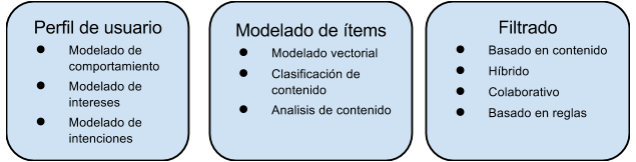
\includegraphics[scale=.75]{images/procrecomendacion.png}
\caption{Proceso de recomendaci\'on según \citep{Gao:2010}}
\label{fig:procrecomendacion}
\end{figure}

\section{Tipos de sistemas de recomendaci\'on}
\label{marco:tecnicasrecomendacion}

En la presente sección se realiza una descripción y clasificación de las distintos tipos de SR basado en el estado del arte \citep{Adomavicius:2005}.

\subsection{Sistemas de recomendaci\'on basados en contenido}
\label{marco:srcontenido}

Se recomienda al usuario un conjunto de ítems basándose en los ítems similares que el usuario ha elegido en el pasado. Este enfoque tiene sus inicios en el área de recuperación de información y filtrado de información, y es usado especialmente en aplicaciones basadas en texto como la recomendación de sitios Web.

Un ítem es representado por un conjunto de \textit{keywords} que son ponderadas usando técnicas como \textbf{TF-IDF} \textit{(Term Frecuency e Inverse Document Frequency)}. Una vez ponderada cada \textit{keyword} se calcula la distancia que tiene cada ítem con los demás mediante alguna medida de similitud (\textit{Pearson}, Coseno, etc).

Los principales problemas que exhiben este tipo de recomendadores son \citep{Adomavicius:2005}:

\begin{itemize}
	\item \textbf{Limitación al análisis del contenido}: estas técnicas están limitadas al conjunto de características que se pueden extraer de los ítems. En algunos casos este problema es complejo, como por ejemplo en imágenes, audio y multimedia.
	\item \textbf{Sobre-especialización}: al usuario solo se le recomendará ítems similares a los que él ha asignado una preferencia alta.  
	\item \textbf{Problema de la partida en frío}: si un usuario no ha valorado un conjunto adecuado de ítems entonces el sistema no es capaz de entregar recomendaciones, ya que no conoce el perfil del usuario.
\end{itemize}

\subsection{Sistemas de recomendaci\'on colaborativos}

Los SR colaborativos se basan en el concepto del ``boca a boca'' y entregan recomendaciones basados en las valoraciones de otros usuarios. En este tipo de SR nace el concepto de capturar la inteligencia colectiva que los usuarios tienen sobre un dominio. En este caso, no se depende del contenido del ítem (es visto como una caja negra). Las fases generales que tienen en común los SR colaborativos basados en valoración numérica son:

\begin{itemize}
\item Ponderar todos los ítems con respecto a la similaridad con el usuario activo.
\item Seleccionar un subconjunto de usuarios para usar como conjunto de predicciones.
\item Normalizar las valoraciones y computar una predicción desde una ponderación combinada de la vecindad del usuario activo.
\end{itemize}

Existen diversas técnicas provenientes del aprendizaje de máquina y la minería de datos para realizar el filtrado. Las técnicas usadas se pueden dividir en dos basadas en heurísticas y en modelo \citep{Adomavicius:2005}.

Las técnicas más usadas dentro del enfoque colaborativo según \citep{Bobadilla:2013} son:
\begin{itemize}
\item \textbf{Vecinos más cercanos \textit{User-user}}: se calcula los usuarios más parecidos al usuario activo y se realiza una predicción de preferencia que el usuario daría a un ítem dadas las preferencias de sus vecinos más cercanos. Este tipo de algoritmo no almacena explícitamente un perfil de usuario, sino que almacena todas las preferencias y vuelve a calcular la lista de vecinos cada vez que se solicitan recomendaciones. Esta técnica  tiene problemas de escalabilidad cuando el número de usuarios crece.

\item \textbf{Vecinos más cercanos \textit{Item-item}}: en este enfoque se calcula para cada ítem sus similares y a partir de este modelo se realiza la predicción al usuario, este enfoque se denomina basado en modelo ya que se genera un modelo de manera \textit{offline}. Para cada ítem se obtienen los $k$ ítems similares, se utiliza para el cálculo de las similitudes las valoraciones comunes de los ítems a comparar. Para calcular la valoración que dará un usuario $u$ a un ítem $i$ se utilizan las valoraciones que el usuario ha dado a ítems vecinos. Se calcula la predicción mediante una suma ponderada.
\end{itemize}

\cite{Su:2009} realizan una revisión de otras técnicas usadas como Redes Bayesianas, Reglas de Asociación, Técnicas de Agrupamiento, Regresiones Lineales, Modelos Probabilísticos, etc.

Algunos de los desafíos de los SR colaborativos se presentan en \citep{Su:2009}:

\begin{itemize}
\item \textbf{Partida en frío de usuarios}: se produce cuando uno o varios usuarios no han valorizado los suficientes ítems para que se le pueda calcular correctamente sus vecinos.
\item \textbf{Partida en frío de ítems}: cuando un ítem se añade al sistema debe ser valorizado antes de poder ser recomendado. 
\item \textbf{Matrices dispersas}: la matriz usuario/ítem es muy dispersa debido a que un conjunto muy pequeño de ítems es usado. El problema es relevante cuando aparece un nuevo usuario en el sistema.
\item \textbf{Escalabilidad}: cuando el número de usuarios e ítems es muy grande los sistemas de recomendación sufren problemas de escalabilidad.
\item \textbf{Sinonimia}: ítems diferentes tienen el mismo contenido o muy similar.
\end{itemize}

\subsection{Sistemas de recomendaci\'on h\'ibridos}
\label{marco:hibridos}

La idea fundamental de los SR híbridos es combinar los enfoques basados en contenido y colaborativos para minimizar las desventajas de cada uno \citep{Burke:2002}. Existen diferentes formas para realizar la hibridación:

\begin{itemize}
	\item Implementar ambos enfoques de forma separada y combinar sus resultados.
	\item Incorporar alguna característica del contenido dentro del enfoque colaborativo o viceversa.
	\item Construir un modelo unificado con características de ambos enfoques.
\end{itemize}

Los SR híbridos son útiles en aplicaciones prácticas donde se debe minimizar las problemáticas inherentes al enfoque basado en contenido y colaborativo.

\section{Sistemas de recomendaci\'on \textit{Context-Aware}}
\label{marco:cars}

Los enfoques existentes para los SR están basados principalmente en el ítem, usuario e  interacciones entre ellos. \cite{Adomavicius:2005} plantean que se debe considerar la información contextual de la interacción como el tiempo, lugar o compañía de otras personas. No es lo mismo recomendar una película para ver el fin semana con la familia o verla solo en el cine un día de semana. Existen varias aplicaciones que requieren de información contextual como por ejemplo la recomendación de vacaciones o eventos. Bajo estas premisas  aparecen los \textbf{CARS} (\textit{Context-aware recommender systems}) para mejorar el proceso de recomendación basándose en cierta información contextual útil \citep{Adomavicius:2011}.

El contexto es un concepto multi-facético estudiado por varias disciplinas de investigación. Cada disciplina tiene su propia idiosincrasia respecto a una definición. Dado que el contexto es variado y tiene múltiples definiciones entonces se considera desde el punto de vista relacionado con los SR que se refiere al contexto de la interacción del usuario. \cite{Adomavicius:2005:2} demuestran la importancia de incluir y usar información contextual en SR . Los autores presentan un enfoque multidimensional que puede mejorar las recomendaciones basándose en información contextual.

Algunos ejemplos de información contextual útil son la ubicación del usuario, las personas que se encuentran cerca, los objetos alrededor, la fecha, día de la semana, estación y temperatura. Luego se aumenta la dimensionalidad del problema de recomendación agregando  dimensiones adicionales a las clásicas ítem-usuario que representan el contexto.

La información contextual se puede obtener de las siguientes formas \citep{Adomavicius:2011}:

\begin{itemize}
\item \textbf{Explícitamente}: se dirige a los usuarios y se le pide información mediante formularios web para elicitar la información. Por ejemplo, ¿Vió  la película en compañía de su novia?
\item \textbf{Implícitamente}: se puede obtener a partir de cambios de la ubicación de los usuarios a través de teléfonos inteligentes, mediante una marca temporal de una operación realizada. La fuente de información se accede directamente, por lo tanto, no existe una interacción con el usuario.
\item \textbf{Infiriendo}: se obtiene información del contexto utilizando métodos estadísticos o de minería de datos.
\end{itemize}

\cite{Adomavicius:2011} señalan que la información contextual se puede aplicar de tres formas en los SR.
\begin{itemize}
	\item \textbf{Pre-filtrado}: se obtienen sólo los eventos relevantes dado un contexto para realizar el cálculo de la recomendación.
	\item \textbf{Dentro del proceso de filtrado}: se agregan las dimensiones de contexto como una nueva variable para el proceso de predicción de valoración.
	\item\textbf{ Post-filtrado}: dado un conjunto de recomendaciones se seleccionan solo las relevantes dado un contexto.
\end{itemize}

Los CARS sitúan los eventos dentro de un espacio de dimensiones que son de utilidad para los SR, cabe destacar que dependiendo de la aplicación se debe validar el conjunto de dimensiones del contexto a usar que aporten de forma positiva al proceso de recomendación \citep{Zhang:2010}.


\section{Informaci\'on social para los SR}
\label{marco:informacionsocial}

Cada vez en la Web 2.0 aparecen nuevas interacciones con los contenidos y entre los usuarios. Estas son por ejemplo \textit{following}, \textit{posting}, \textit{blogging}, \textit{rating} y \textit{tagging} entre otros. Estas interacciones son denominadas información social.

La información social se usa con tres objetivos \citep{Bobadilla:2013}:

\begin{enumerate}
	\item Mejorar la calidad de las recomendaciones y predicciones.
	\item Proponer y generar nuevos SR.
	\item Dilucidar las relaciones más importantes entre la información social y el proceso colaborativo.
\end{enumerate}

La confiabilidad y reputación de los usuarios de una red social se ha estudiado con el objetivo de generar medidas que permitan calcular la credibilidad del usuario a través de información implícita o explícita de este \citep{Victor:2011}.

El etiquetado social (\textit{tags}) se refiere al proceso de asignar etiquetas que tienen sentido para el usuario (folksonomía). De esta forma, un comportamiento de etiquetado hacia un documento se puede modelar como un evento representado usando una tripleta (usuario, ítem, etiqueta).  El etiquetado social puede ser usado para mejorar el filtrado colaborativo  utilizándose como un nuevo tipo de interacción del usuario hacia los ítems \citep{Bobadilla:2013} o para sugerir etiquetas útiles e informativas para un ítem emergente, basado en información histórica \citep{Song:2011}. 

\section{3-Ontology}
\label{marco:3ontology}

El área de investigación de la \textbf{CSCW} (\textit{Computer-supported cooperative work}) es un campo interdisciplinario estudiado por economistas, sociólogos, antropólogos, psicólogos, ingenieros, etc. En este contexto \cite{Leiva:2002} plantean la \textit{3-Ontology}, un \textit{framework} que tiene como objetivo soportar el \textit{“Cooperative Awareness”} (darse-cuenta colaborativo), que permite modelar el contexto de trabajo o lúdico donde las personas ubican las acciones propias y las de los demás.

La \textit{3-ontology} es un \textit{framework} conceptual que modela el ``darse-cuenta colaborativo'', por lo tanto modela el ``contexto'' de cualquier interacción que tenga un valor colaborativo. Se definen 3 conceptos que construyen sentido para los usuarios: comunidades, eventos y lugares. Se considera el  darse-cuenta como una relación sistemáticamente dependiente entre estos conceptos. No existe una jerarquía entre estos conceptos dado que se co-definen entre sí. En otras palabras, el contexto donde colaboran los usuarios está ``situado'' en un espacio, tiempo y cultura.

\cite{Leiva:2002} definen los siguientes 3 contenedores se sentido para la \textit{3-Ontology}:

\begin{enumerate}
	\item \textbf{Comunidades}: corresponde a un conjunto de usuarios que habita un lugar que son protagonistas de los eventos. La comunidad es representada mediante retratos que representan la composición de estas mediante usuarios y comunidades.
	\item  \textbf{Lugares}: pueden constituir un espacio físico o virtual. En estos habitan los objetos a los cuales se efectúan eventos. Son representados mediante mapas que pueden ser de naturaleza electrónica o física.
	\item \textbf{Eventos}: son de carácter colaborativo. Estos eventos están situados en un tiempo y lugar. Son representados mediante trazas que muestran el contexto histórico en que adquieren sentido. Un evento puede ser atómico o compuesto (conjunto de eventos que tienen un significado común).
\end{enumerate}

Una representación basada en la \textit{3-ontology} permite explicitar el ``valor'' colaborativo de las interacciones. Luego una interacción sucede en un lugar, es efectuado por un usuario que pertenece a una comunidad, en un tiempo determinado, en un lugar, etc. En la Figura \ref{fig:diagram3ontology} se muestran las relaciones que existen entre los conceptos de la \textit{3-ontology}:
\begin{itemize}
 \item Los objetos pertenecen a los lugares, mientras que los usuarios a comunidades. 
 \item Los eventos son realizados sobre objetos de un lugar efectuados por usuarios de una comunidad.
 \item Las comunidades habitan un lugar y participan de los eventos.
 \item Los lugares pertenecen a comunidades y sitúan los eventos.
 \item Los tres contenedores de sentido pueden ser constituidos de forma recursiva.
\end{itemize}


\begin{figure}[tp]
\centering
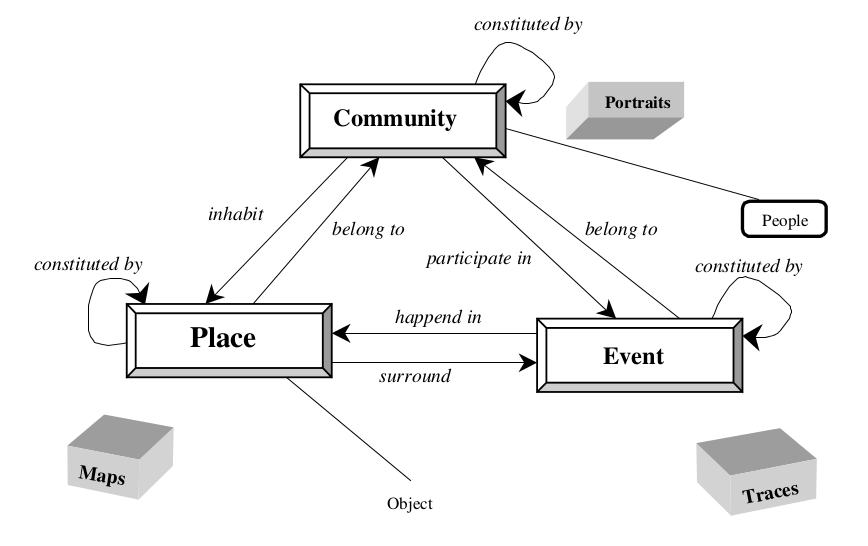
\includegraphics[scale=.5]{images/locus3ontology.png}
\caption{Diagrama conceptual \textit{3-Ontology} \citep{Leiva:2002}}
\label{fig:diagram3ontology}
\end{figure}

\subsection{Darse-cuenta de la historia}

Las trazas denotan la relación existente entre los eventos efectuados. Es un orden parcial (representado mediante) de los eventos efectuados por un usuario o un conjunto de usuarios. Las trazas agregan continuidad en el desarrollo de flujos de trabajo. Para soportar este darse-cuenta se pueden representar al menos 2 tipos de servicios:

\begin{itemize}
\item \textbf{Notificación}: se refiere a servicios que permiten mantener al usuario consciente del contexto dadas las trazas de eventos.
\item \textbf{Continuidad}: se refiere a servicios que permitan la continuidad de las actividades que pueda estar realizando un usuario particular.
\end{itemize}

\subsection{Darse-cuenta de la presencia}

Los mapas representan la constitución de los lugares donde suceden los eventos. Permite a los usuarios ver donde ocurren los eventos, que objetos estuvieron involucrados, personas, etc. Para soportar el darse-cuenta de la presencia se pueden representar dos tipos de servicios.

\begin{enumerate}
\item \textbf{Conectividad}: este tipo de servicios responde a la siguiente pregunta ¿Quiénes están alrededor y que están haciendo?. Si el evento ocurre dentro de un espacio virtual entonces se pueden proveer servicios de conexión entre usuarios. La proximidad física puede generar posibilidades de interacción \citep{Leiva:2002}.
\item \textbf{Disponibilidad}: esta clase de servicios responde a las siguientes preguntas tales como ¿Qué hay en este lugar?, ¿Qué está sucediendo en este lugar?.
\end{enumerate}

\subsection{Darse-cuenta de los usuarios}

Los retratos representan a comunidades (conjuntos de usuarios) y conjunto de comunidades. Determinan la identidad de los usuarios, afinidad entre estos, pueden ser explícitas (los usuarios determinan por su propia voluntad estar en una comunidad) o implícitas (dado el comportamiento del usuario se infiere que es parte de una comunidad). Los servicios que prestan los retratos son los siguientes:

\begin{enumerate}
\item \textbf{Identidad}: permite a un usuario saber qué usuarios son similares a él y a qué comunidad pertenece.
\item \textbf{Expansibilidad}: es la capacidad de una comunidad de ir creciendo o disminuyendo sus miembros en el tiempo. Estos conceptos implican algunos criterios de cohesión y adhesión de la comunidad, temas que pueden ser numéricamente representados.
\end{enumerate}

Para implementar los servicios de darse-cuenta colaborativo \cite{Leiva:2002} proponen una arquitectura denominada \textit{JAZZ}. Esta se compone de servidores que implementan los servicios de darse-cuenta para que sean usados por aplicaciones colaborativas. En otras palabras se construye una arquitectura clásica de dos capas: base de datos y servicios. Dadas estas premisas, en este trabajo de tesis solo se utilizan las representaciones (trazas, mapas y retratos) dotadas de lógica mediante la agregación de métodos, por lo que pueden ser vistos como objetos que tienen un comportamiento propio. Luego se debe explicitar que no se implementan servicios de darse-cuenta colaborativo en servidores como lo proponen \cite{Leiva:2002}.

La \textit{3-Ontology} es un \textit{framework} conceptual, por lo tanto, no corresponde a una ontología de índole informático que define un conjunto de entidades y relaciones entre ellas para un dominio específico \citep{Leiva:2002}. Sin embargo, es una base conceptual que permite modelar ontologías para dominios específicos. En otras palabras la \textit{3-ontology} se puede considerar como una meta-ontología para describir dominios colaborativos diversos.

%\section{Resumen}
%
%En este capítulo se realizó una revisión de los fundamentos teóricos del trabajo de tesis propuesto. Para comenzar se definieron los SR y sus características. Luego se presentó una categorización de los SR basada en el estado del arte. Posteriormente se definieron los ``\textit{Context-Aware Recommender Systems}'' que son SR que utilizan información contextual para realizar el cálculo de las recomendaciones. También se define la información social que es utilizada por los SR como es el caso de las etiquetas. Finalmente, se presentó el \textit{framework} conceptual \textit{3-Ontology} que permite situar las interacciones de ambientes colaborativos en tres dimensiones tiempo, espacio y sociedad.









